\documentclass[11pt]{article}
\usepackage{amsmath, amssymb, amscd, amsthm, amsfonts}
\usepackage{graphicx}
\usepackage{hyperref}
\hypersetup{
    colorlinks=true,
    linkcolor=blue,
    filecolor=magenta,      
    urlcolor=cyan,
    pdftitle={Overleaf Example},
    pdfpagemode=FullScreen,
    }
\usepackage[dvipsnames]{xcolor}

\oddsidemargin 0pt
\evensidemargin 0pt
\marginparwidth 40pt
\marginparsep 10pt
\topmargin -20pt
\headsep 10pt
\textheight 8.7in
\textwidth 6.65in
\linespread{1.2}

\title{Course Report: Unsupervised Learning}
\author{Nan He}
\date{}

\newtheorem{theorem}{Theorem}
\newtheorem{lemma}[theorem]{Lemma}
\newtheorem{conjecture}[theorem]{Conjecture}

\newcommand{\rr}{\mathbb{R}}

\newcommand{\al}{\alpha}
\DeclareMathOperator{\conv}{conv}
\DeclareMathOperator{\aff}{aff}

\begin{document}

\maketitle

%\begin{abstract}
%(Abs)
%\end{abstract}

\section{Main objective of the analysis}\label{section-introduction-1}
Acknowledgement: this is a course project for \href{https://www.coursera.org/professional-certificates/ibm-machine-learning}{IBM Machine Learning professional certificate}. The project notebook can be accessed \href{https://github.com/henankf223/Assignment_3/blob/cddb6fe0d2dcb9b413ce74028301c65b87316e8b/Assignment_Classification.ipynb}{here}.

In this report, the data I will be using is a Customer Personality Analysis data set from Kaggle, the link for the data set is \href{https://www.kaggle.com/imakash3011/customer-personality-analysis}{here}.
The goal of this report is to segment the customer using unsupervised learning techniques. 

The target includes: \\
1) Find clusters of customers that share similar characteristics. \\
2) Interpret the clustering results, create portraits for each group of customers. \\
3) Evaluate the performance of the clustering algorithms. \\

\section{Description of the data set}\label{section-introduction-2}
The data set is a surveying result of 2140 customers for a grocery store. 
The feature columns are in four categories:

\begin{itemize}
\item People

ID: Customer's unique identifier\\
Year\_Birth: Customer's birth year\\
Education: Customer's education level\\
Marital\_Status: Customer's marital status\\
Income: Customer's yearly household income\\
Kidhome: Number of children in customer's household\\
Teenhome: Number of teenagers in customer's household\\
Dt\_Customer: Date of customer's enrollment with the company\\
Recency: Number of days since customer's last purchase\\
Complain: 1 if the customer complained in the last 2 years, 0 otherwise

\item Products

MntWines: Amount spent on wine in last 2 years\\
MntFruits: Amount spent on fruits in last 2 years\\
MntMeatProducts: Amount spent on meat in last 2 years\\
MntFishProducts: Amount spent on fish in last 2 years\\
MntSweetProducts: Amount spent on sweets in last 2 years\\
MntGoldProds: Amount spent on gold in last 2 years

\item Promotion

NumDealsPurchases: Number of purchases made with a discount\\
AcceptedCmp1: 1 if customer accepted the offer in the 1st campaign, 0 otherwise\\
AcceptedCmp2: 1 if customer accepted the offer in the 2nd campaign, 0 otherwise\\
AcceptedCmp3: 1 if customer accepted the offer in the 3rd campaign, 0 otherwise\\
AcceptedCmp4: 1 if customer accepted the offer in the 4th campaign, 0 otherwise\\
AcceptedCmp5: 1 if customer accepted the offer in the 5th campaign, 0 otherwise\\
Response: 1 if customer accepted the offer in the last campaign, 0 otherwise

\item Place

NumWebPurchases: Number of purchases made through the company’s website\\
NumCatalogPurchases: Number of purchases made using a catalogue\\
NumStorePurchases: Number of purchases made directly in stores\\
NumWebVisitsMonth: Number of visits to company’s website in the last month

\end{itemize}

\newpage

The data types are:

\begin{figure}[h!]
\centerline{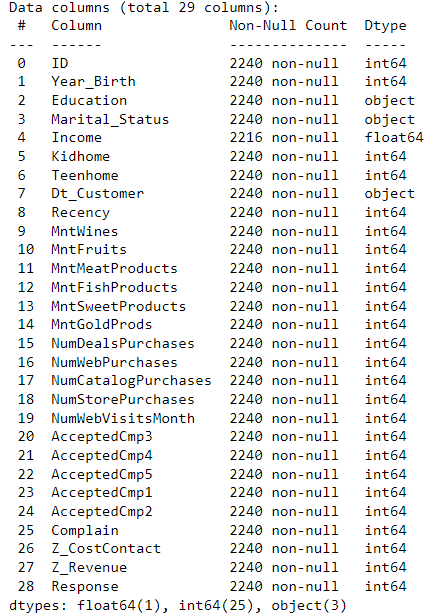
\includegraphics[scale=0.5]{clu_1.png}}
\caption{Initial data types.}
\end{figure}

\section{Data exploration, cleaning, and feature engineering}\label{section-introduction-3}
The data need to be cleaned. Here is the list of actions I took:

\begin{itemize}
\item Drop "ID", "Z\_Revenue", "Z\_CostContact".
Since they are not related with our goal.
\item Fill NaN values in "Income" with the median of income. 
The assumption is that a random people have the highest possibility to have incomes around the median.
\item Encode "Martial Status" and "Education" to numeric variables. 
To reduce the number of possible values, I will only consider "Single" and "Not Single" for "Martial Status", and "Low", "Medium", "High" for "Education". All original values will be assigned into those new categories.
\item Create "Customer\_days" to replace the "Dt\_Customer".
This will be done by first convert "Dt\_Customer" to pandas date-time format, then use the latest date in the data minus every date-time values. The resulting "Customer\_days" will be a new feature with value between 0 and 720 days.
\end{itemize}

The data after cleaning contains 25 features, of which one is float64, and others are all int64.
Here is the correlation heat-map for all numerical variables:

\begin{figure}[h!]
\centerline{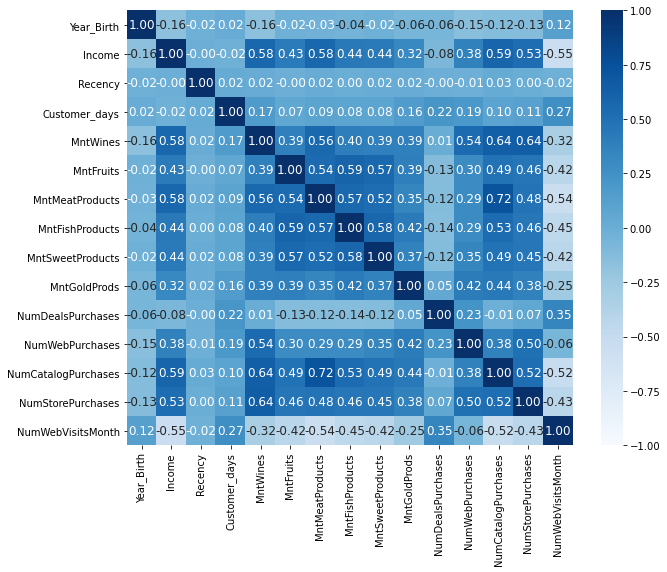
\includegraphics[scale=0.7]{clu_2.png}}
\caption{Correlation Heatmap.}
\end{figure}

There are some interesting observations here, for example:
\begin{itemize}
\item Time-related features, including "Year\_Birth", "Recency", and "Customer\_days", have very weak correlation with other features.
\item "Income" is positively correlated with every type of consumption, but negatively correlated with "Year\_Birth", "NumDealsPurchases", and "NumWebVisitsMonth".
\end{itemize}

\section{Dimensionality Reduction}\label{section-model}
In this section, I will start building an unsupervised model to segment the customers.
Since there are 25 features, a direct clustering will end up into curse of dimensionality.
There are also many encoded categorical features, whose distance do not have actual meanings.
Therefore, it is important to first perform PCA to transform the features into principle components.
The steps include:
\begin{itemize}
\item Scale the data using RobustScalar, since there are many outliers.
\item Compute and transform the features using PCA, truncated at 2 principle components.
\end{itemize}
The resulting data are shown below:

\begin{figure}[h!]
\centerline{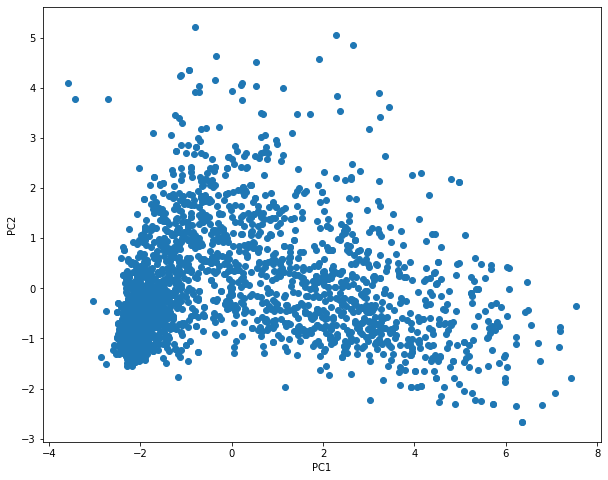
\includegraphics[scale=0.6]{clu_3.png}}
\caption{Data distribution after PCA.}
\end{figure}

\section{Testing different clustering models}\label{section-model}
Here I will test multiple clustering models.
The clustering results are plotted for every parameters below.
The model will be evaluated using \\
1) Silhouette score: higher value indicates better defined clusters. \\
2) Davies-Bouldin score: lower value indicates better cluster separation:

\newpage

\begin{itemize}
\item \textbf{Kmeans clustering}, $k=4$ is decided using elbow method.
\begin{figure}[h!]
\centerline{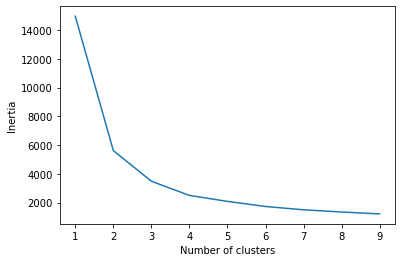
\includegraphics[scale=0.5]{clu_4.png}}
\caption{Kmeans elbow curve.}
\end{figure}

\begin{figure}[h!]
\centerline{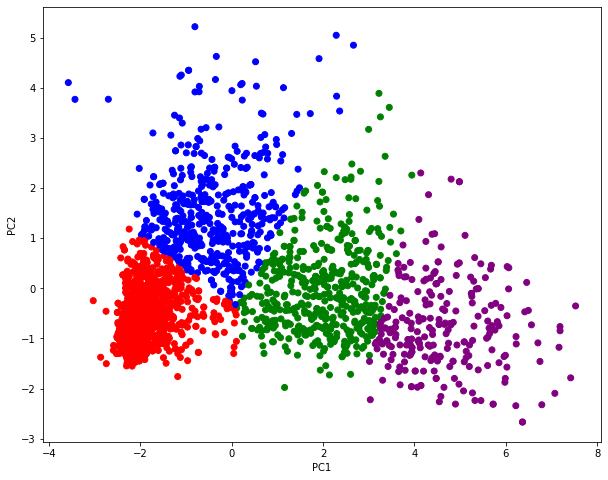
\includegraphics[scale=0.5]{clu_5.png}}
\caption{Kmeans clustering result.}
\end{figure}

\newpage

\item \textbf{Single-linkage agglomerative clustering}, using $k=4$.

\begin{figure}[h!]
\centerline{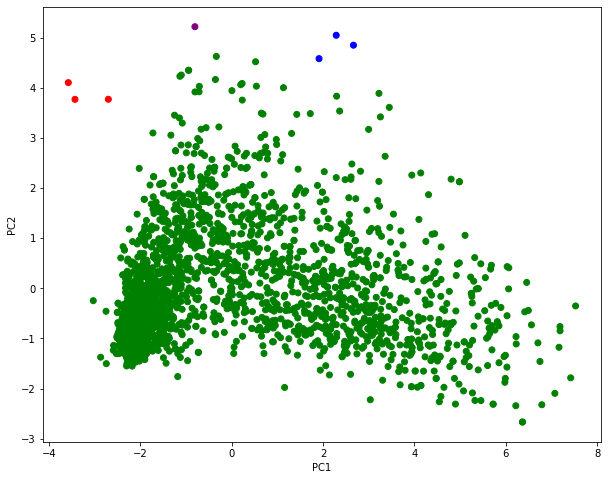
\includegraphics[scale=0.5]{clu_6.png}}
\caption{Single-linkage agglomerative clustering result.}
\end{figure}

\item \textbf{Average-linkage agglomerative clustering}, using $k=4$.

\begin{figure}[h!]
\centerline{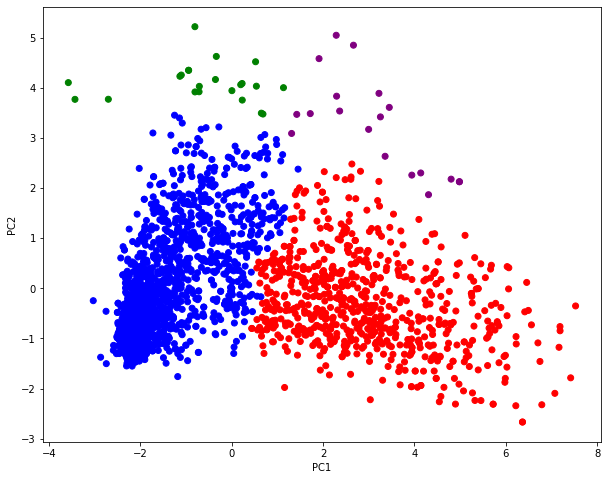
\includegraphics[scale=0.5]{clu_7.png}}
\caption{Average-linkage agglomerative clustering result.}
\end{figure}

\newpage

\item \textbf{Ward-linkage agglomerative clustering}, using $k=4$.

\begin{figure}[h!]
\centerline{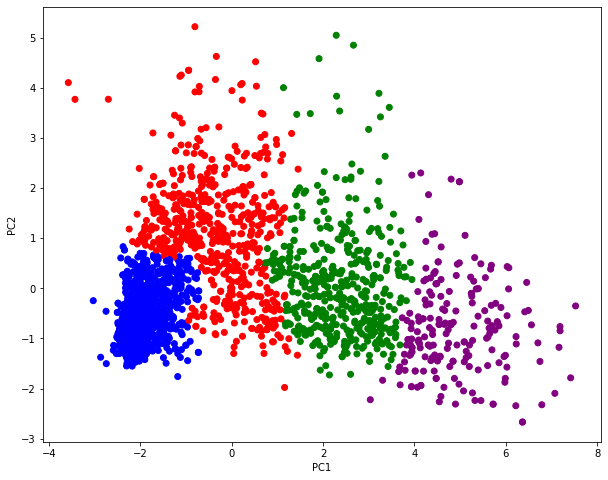
\includegraphics[scale=0.5]{clu_8.png}}
\caption{Ward-linkage agglomerative clustering result.}
\end{figure}

\item \textbf{Complete-linkage agglomerative clustering}, using $k=4$.

\begin{figure}[h!]
\centerline{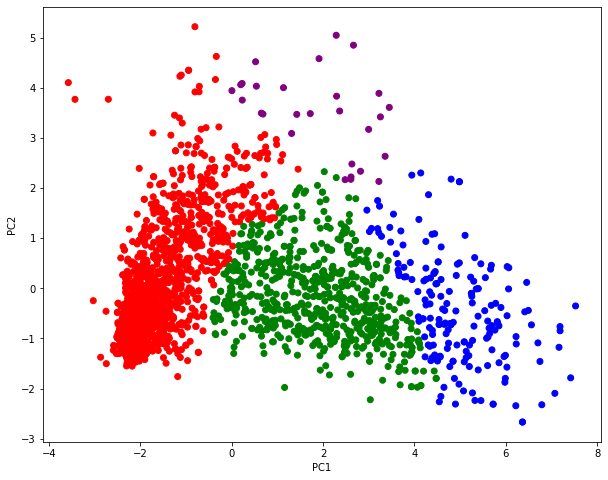
\includegraphics[scale=0.5]{clu_9.png}}
\caption{Complete-linkage agglomerative clustering result.}
\end{figure}

\newpage

\item \textbf{DBSCAN}, using $\epsilon=0.1$.

\begin{figure}[h!]
\centerline{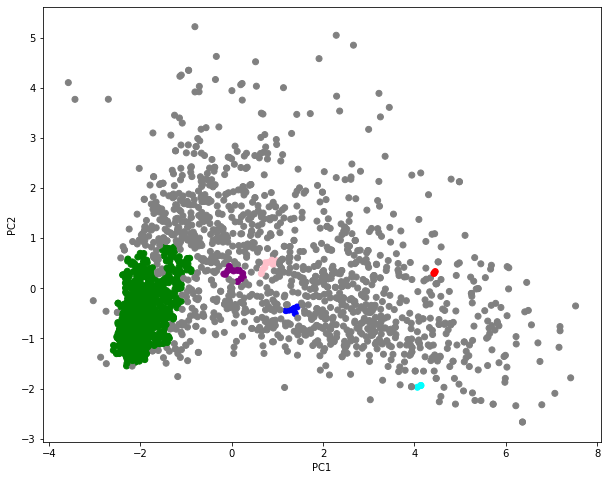
\includegraphics[scale=0.5]{clu_10.png}}
\caption{DBSCAN result 1, not all clusters are colored.}
\end{figure}

\item \textbf{DBSCAN}, using $\epsilon=0.5$.

\begin{figure}[h!]
\centerline{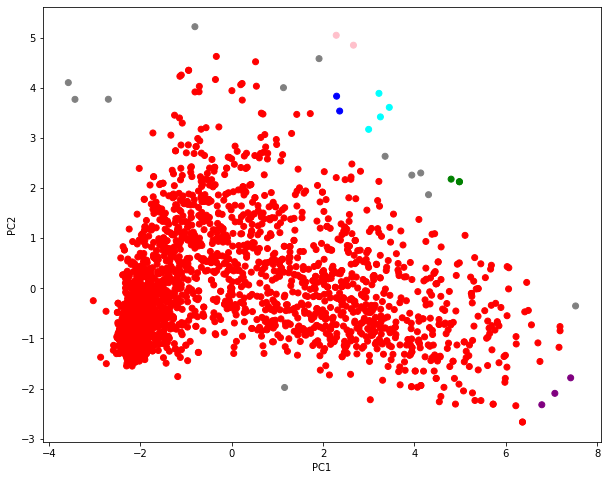
\includegraphics[scale=0.5]{clu_11.png}}
\caption{DBSCAN result 2, not all clusters are colored.}
\end{figure}

\end{itemize}

\newpage

The scores for each model is listed below.

\begin{table}[h]
\begin{tabular}{lll}
\hline
\hline
Method           & Silhouette score & Davies-Bouldin score \\
\hline
Kmeans           & 0.497            & 0.786                \\
Single-linkage   & 0.325            & 0.499                \\
Average-linkage  & 0.500            & 0.716                \\
Ward-linkage     & 0.466            & 0.833                \\
Complete-linkage & 0.457            & 0.771                \\
DBSCAN $\epsilon=0.1$ & -0.083           & 1.951                \\
DBSCAN $\epsilon=0.5$ & 0.186            & 1.639                \\
\hline
\hline
\end{tabular}
\end{table}

\section{Final model choices and analysis}\label{section-pred}
From the scatter plots and the scores, the observations are
\begin{itemize}
\item Kmeams works well in this case, creating very balanced clusters.
\item Single-linkage agglomerative clustering provide the best separation between clusters (lowest Davies-Bouldin score), however, its clusters are very dispersed and ill-defined.
\item In my case, DBSCAN struggles to find correct clusters no matter what $\epsilon$ I chose. One possible reason is that the data itself has various densities for different regions, which plaguing density-based methods.
\item The best performance comes from Average-linkage agglomerative clustering, which will be the model I use for the following analysis.
\end{itemize}

\section{Key Findings and Insights}\label{section-find}
Let's dive into the results of Average-linkage agglomerative clustering, and see what this segmentation tells us.
I put the predicted labels back to the dataframe, and investigate the distribution of different features among clusters.

\newpage

\begin{itemize}
\item Income.

\begin{figure}[h!]
\centerline{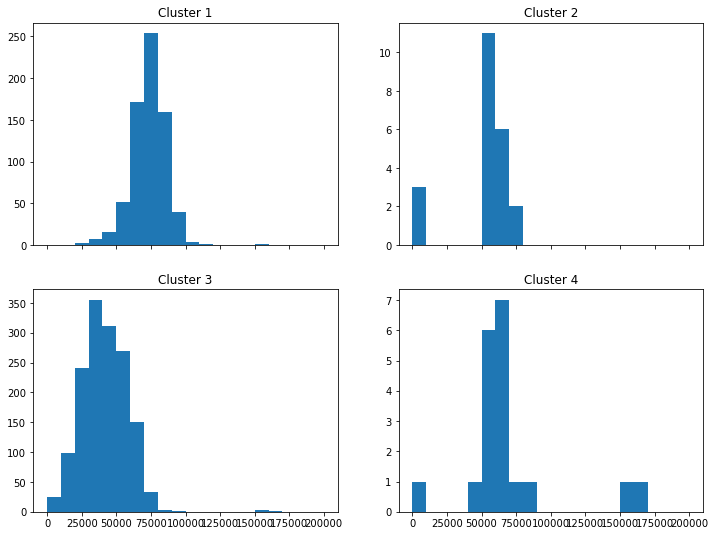
\includegraphics[scale=0.4]{clu_conc_1.png}}
\caption{Income of different clusters.}
\end{figure}

Since only cluster 1 and 3 have significant number of labels, in the following plot, I will focus only on cluster 1 and 3.

\item Education.

\begin{figure}[h!]
\centerline{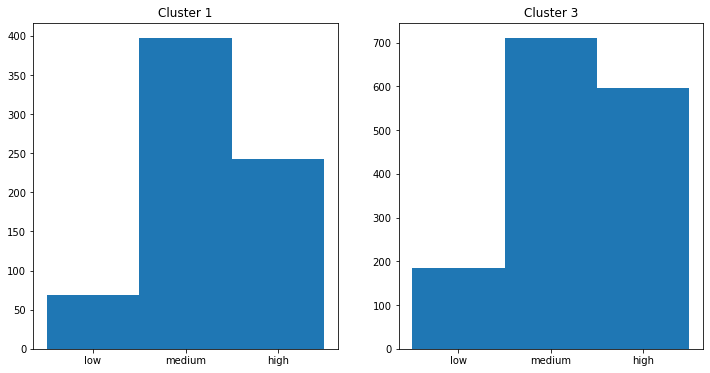
\includegraphics[scale=0.35]{clu_conc_2.png}}
\caption{Education level of different clusters.}
\end{figure}

\newpage

\item Marital Status.

\begin{figure}[h!]
\centerline{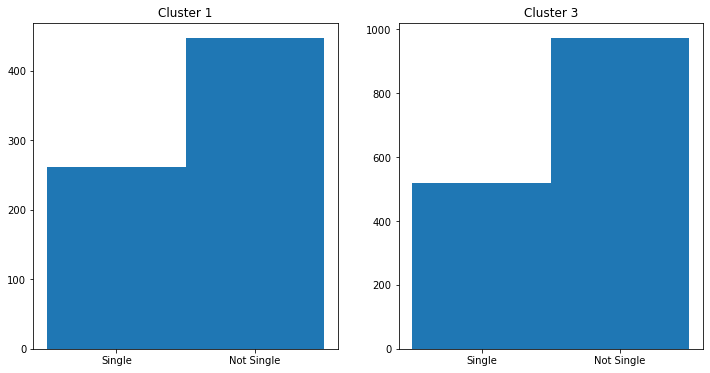
\includegraphics[scale=0.35]{clu_conc_3.png}}
\caption{Marital Status of different clusters.}
\end{figure}

\item Year of birth.

\begin{figure}[h!]
\centerline{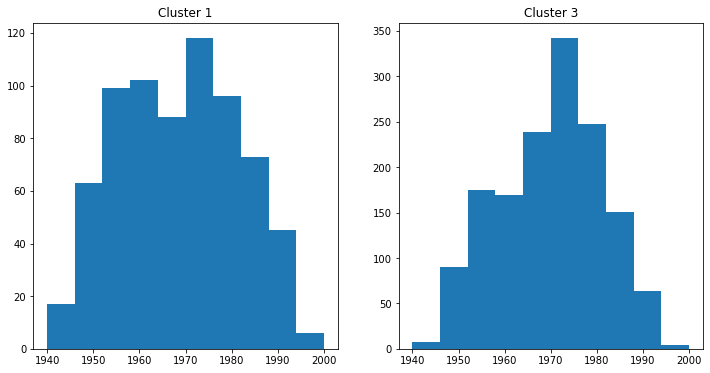
\includegraphics[scale=0.35]{clu_conc_4.png}}
\caption{Birth year of different clusters.}
\end{figure}

\item Meat purchases.

\begin{figure}[h!]
\centerline{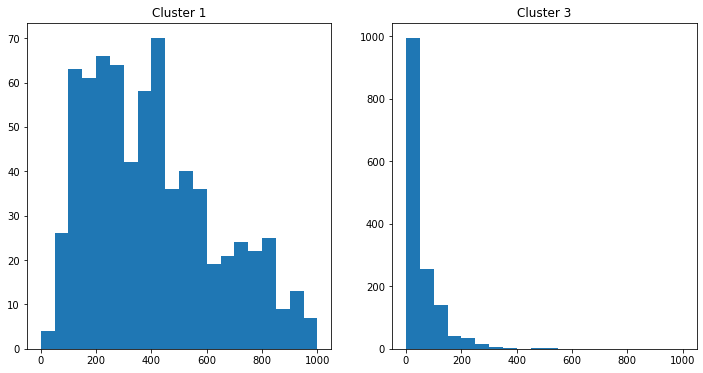
\includegraphics[scale=0.35]{clu_conc_5.png}}
\caption{Meat purchases of different clusters.}
\end{figure}

\newpage

\item Wine purchases.

\begin{figure}[h!]
\centerline{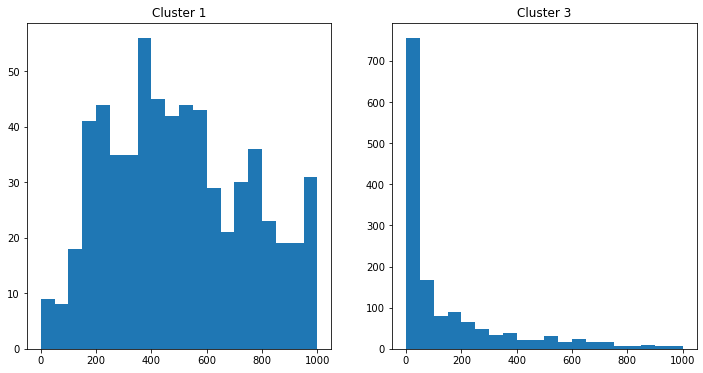
\includegraphics[scale=0.35]{clu_conc_6.png}}
\caption{Wine purchases of different clusters.}
\end{figure}

\item Fruit purchases.

\begin{figure}[h!]
\centerline{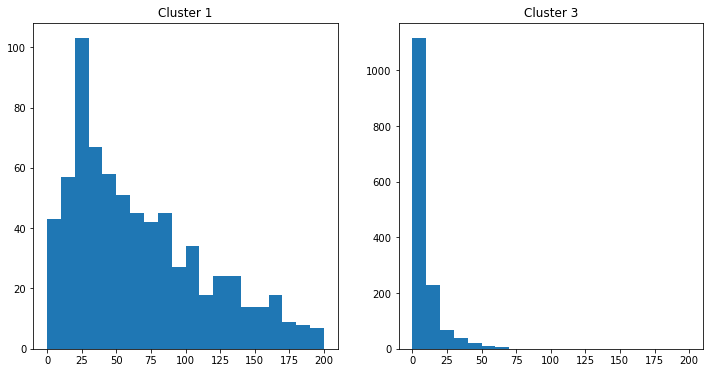
\includegraphics[scale=0.35]{clu_conc_7.png}}
\caption{Fruit purchases of different clusters.}
\end{figure}

\item Number of purchases using deals.

\begin{figure}[h!]
\centerline{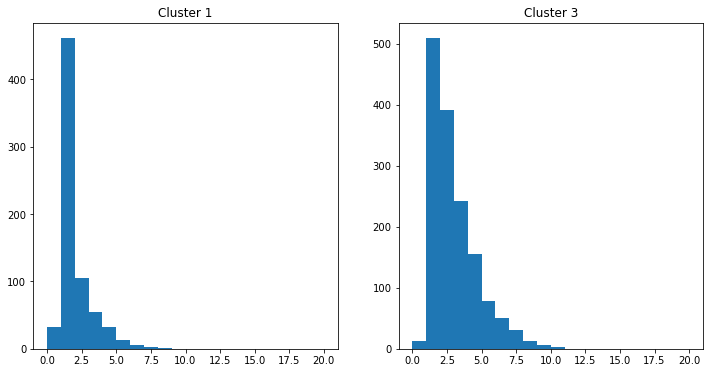
\includegraphics[scale=0.35]{clu_conc_8.png}}
\caption{Number of purchases using deals for different clusters.}
\end{figure}

\newpage

\item Number of purchases through web.

\begin{figure}[h!]
\centerline{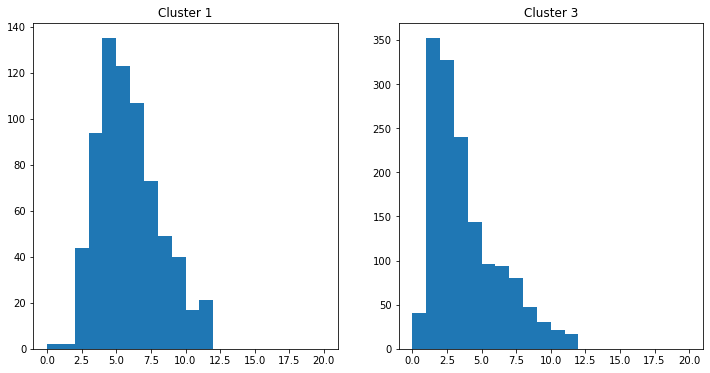
\includegraphics[scale=0.35]{clu_conc_9.png}}
\caption{Number of purchases through web for different clusters.}
\end{figure}

\item Number of purchases at store.

\begin{figure}[h!]
\centerline{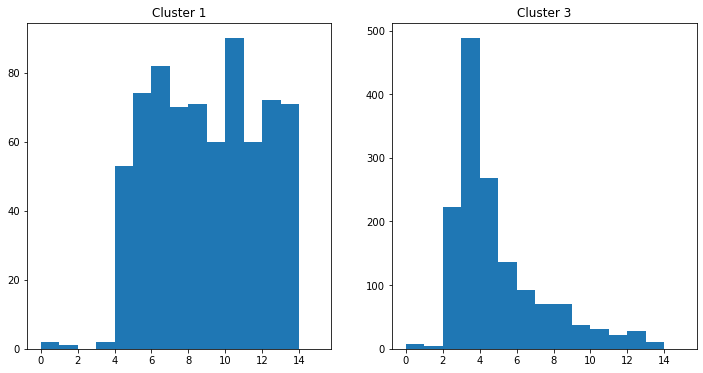
\includegraphics[scale=0.35]{clu_conc_10.png}}
\caption{Number of purchases at store for different clusters.}
\end{figure}

\item Number of website visits.

\begin{figure}[h!]
\centerline{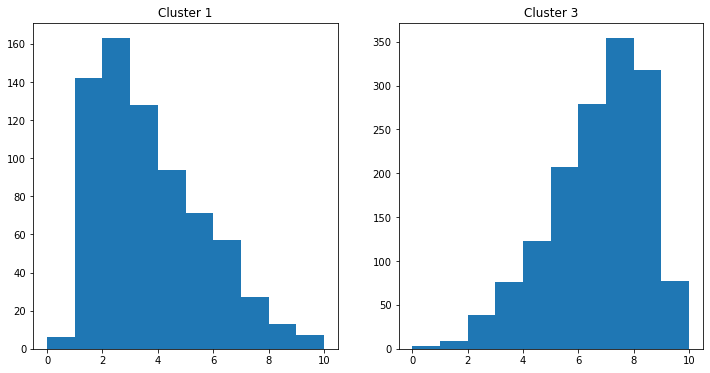
\includegraphics[scale=0.35]{clu_conc_11.png}}
\caption{Number of website visits for different clusters.}
\end{figure}

\newpage

\end{itemize}

From those histograms, I find that most customers (98\%) fall into two categories, with less than 2\% being outliers.
The portrait of those two type of customers are:

\begin{itemize}
\item Cluster 1: those customers have higher average income, older (in average), purchase more meat, wine, fruits, use fewer deals, and prefer shopping at store.
\item Cluster 3: those customers have lower average income, younger, purchase fewer goods, tend to use more deals, prefer shopping through website, and visit the website more frequently.
\item Other features are not significantly different among clusters.
\end{itemize}

\section{Summary and suggestions for next steps}\label{section-sugg}
In summary, this report perform a customer segmentation for a survey data set. By using PCA and clustering algorithms, I find two major customer types. Those insights will be helpful for the store to target there customers.

One fallacy is that in my report, for simplicity, I truncate the features to only 2 principle components. This action may cause large residuals, where many other contributing factors are ignored. For example, in my clustering, it seems that Education have no impact on the segmentation, which is non-intuitive.

The next steps may be:
\begin{itemize}
\item Use different number of principle components and compute the residuals of the decomposition to find a best balance.
\item Try kernel PCA and other dimensionality reduction techniques.
\item Try to find more balanced segmentations, like 4 medium-sized clusters, which will provide us more information on customer personality.
\end{itemize}

%\bibliographystyle{alpha}
%\bibliography{references} % see references.bib for bibliography management

\end{document}
